\normalfalse \difficiletrue \tdifficilefalse
\correctiontrue

%\UPSTIidClasse{11} % 11 sup, 12 spé
%\newcommand{\UPSTIidClasse}{12}

\exer{Pompe à piston axial  $\star$ \label{C2:06:11}}
\setcounter{numques}{0}
\UPSTIcompetence[2]{C2-06}
\index{Compétence C2-06}
\index{Pompe à pistons radiaux}
\index{Arbre à cames}
\ifcorrection
\else
\textbf{Pas de corrigé pour cet exercice.}
\fi

\ifprof
\else
Soit le mécanisme suivant. On a $\vect{AB}=e\vect{i_1}$ et $\vect{BI}=R\vect{j_0}$ et $\vect{AC}=\lambda(t)\vect{j_0}$. De plus, 
$e=\SI{10}{mm}$ et $R=\SI{20}{mm}$. Le contact entre \textbf{1} et \textbf{2} en $B$ est maintenu en permanence par un ressort suffisamment raide (non représenté) positionné entre \textbf{0} et \textbf{2}. 
\begin{center}
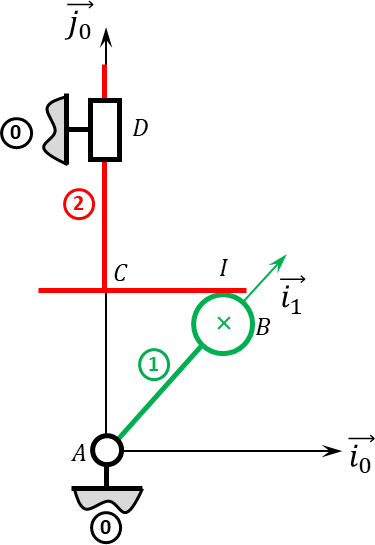
\includegraphics[width=\linewidth]{11_01}
\end{center}
\fi

\question{Tracer le graphe des liaisons.}

\ifprof
\begin{center}
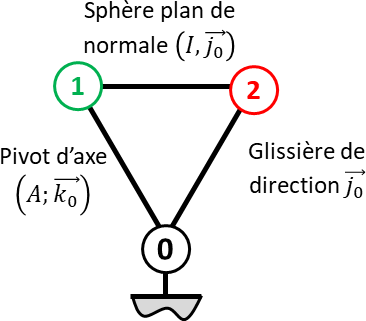
\includegraphics[width=.3\linewidth]{11_01_c}
\end{center}

\else
\fi

\question{Exprimer $\lambda(t)$ en fonction de $\theta(t)$.}

\ifprof

En écrivant la fermeture géométrique, on a $\vect{AB}+\vect{BI}+\vect{IC}+\vect{CA}=\vect{0}$.

On a donc, $e\vi{1}+R\vj{0}+\mu\vi{0}-\lambda(t)\vj{0}=\vect{0}$. En projetant l'expression sur $\vj{0}$ (dans ce cas, l'expression suivant $\vi{0}$ n'est pas utile) :
$ e\sin\theta +R - \lambda(t)=0$.

On a donc, $\lambda(t)=e\sin\theta +R $.
\else
\fi

\question{Exprimer $\dot{\lambda}(t)$ en fonction de $\dot{\theta}(t)$.}
\ifprof

En dérivant l'expression précédente, on a $\lambdap (t)=e\thetap(t) \cos\theta (t) $.
\else
\fi

\question{On note $S$ la section du piston \textbf{2}. Exprimer le débit instantané de la pompe.}
\ifprof

En notant $q(t)$ le débit instantané, $q(t)=eS\thetap(t) \cos\theta (t)$.
\else
\fi

\question{En utilisant Python, tracer le débit instantané de la pompe pour un tour de pompe pour $e=\SI{10}{mm}$ et $R=\SI{10}{mm}$ ainsi que pour $e=\SI{20}{mm}$ et $R=\SI{5}{mm}$. La fréquence de rotation est $\dot{\theta}(t)=\SI{100}{rad.s^{-1}}$, la section du piston est donnée par $S=\SI{1}{cm^2}$.}
\ifprof

\noindent\hrule
\begin{lstlisting}
#!/usr/bin/env python
# -*- coding: utf-8 -*-

"""11_PompePistonAxial.py"""

__author__ = "Xavier Pessoles"
__email__ = "xpessoles.ptsi@free.fr"

import numpy as np
import matplotlib.pyplot as plt
import math as m
from scipy.optimize import newton
from scipy.optimize import fsolve

R = 0.02 # m
e = 0.01 # m

def calc_lambda(theta):
    res= e*np.sin(theta)+R
    
    return res

def calc_lambdap(theta,w):
   
    res = e*w*np.cos(theta)
    return res

def plot_debit():
    plt.cla()
    w = 100 # rad/s 
    les_t = np.linspace(0,0.1,1000)
    les_theta = w*les_t
    global e 
    S = 1e-4
    e = 20e-3
    les_q = e*S*w*np.cos(les_theta)
    plt.plot(les_t,les_q)
    plt.xlabel("Temps (s)")
    plt.ylabel("Débit (${m}^3s^{-1}$)")
    plt.grid()
    plt.savefig("11_02_c.png")
    plt.show()
    
plot_debit()
\end{lstlisting}
\noindent\hrule

\begin{center}
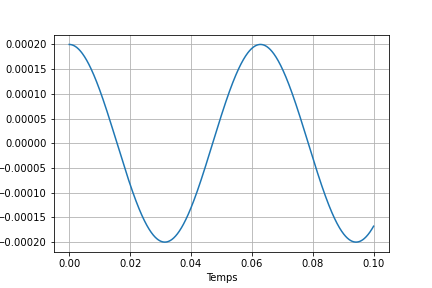
\includegraphics[width=.5\linewidth]{11_02_c}
\end{center}

\else
\fi




\ifprof
\else
\footnotesize
\ifcolle
\else
\begin{center}
\begin{tabular}{|p{.9\linewidth}|}
\hline
Indications :
\begin{enumerate}
\item .
\item $ e\sin\theta +R - \lambda(t)=0$.
\item $\lambdap (t)=e\thetap(t) \cos\theta (t) $.
\item $q(t)=eS\thetap(t) \cos\theta (t)$.
\item .
\end{enumerate} \\ \hline
\end{tabular}
\end{center}
\fi
\normalsize
\begin{flushright}
\footnotesize{Corrigé  voir \ref{C2:06:11}.}
\end{flushright}%
\fi